\chapter{Applicativo}

\section{Struttura}

L'applicativo è sviluppato in Python usando la libreria grafica
PyQt versione 5.
La scelta è ricaduta su essa per la sua semplicità d'uso,
l'ergonomia di sviluppo ed il fatto che gli interpreti
Python siano {\it cross-platform}, ovvero lo stesso codice
possa essere utilizzato su vari sistemi operativi.

Ai fini di testare l'applicativo sarebbe necessario
avere a disposizione un dispositivo ISCAN da poter collegare
al computer e vedere il comportamento dell'applicativo con
la sorgente audio ricevuta.
Questo è ovviamente impratico per una lunga serie di motivi,
dal dover impegnare lo strumento per lunghi periodi di tempo
alla necessità di avere un paziente che si stia sottoponendo
ad un esame in modo da avere un responso.
Tuttavia su piattaforme Linux, con sicuramente altre opzioni
possibili per sistemi Windows e macOS, è possibile simulare
una sorgente video che in realtà non esiste, grazie alle API
di sistema {\it Video for Linux 2} (V4L2) e al software
FFMPEG.

Nella pratica quel che si fa è utilizzare V4L2 in modo da
simulare a livello sistema operativo un dispositivo video che
in realtà non esiste.
Il sistema operativo crea comunque un file che lo rappresenta
su cui grazie ad FFMPEG e ad un suo apposito modulo per V4L2
si va a scrivere su tale file un video in maniera ciclica,
in modo che questa sorgente sia esattamente come una che
potrebbe venire da un dispositivo video qualunque, come una
webcam, un cavo HDMI o lo stesso ISCAN.
Il video in questione è ovviamente un video di un'endoscopia
ottenuto dal dataset HyperKvasir.

La fase di {\it serving} del modello, ovvero quella in cui esso
viene esposto in modo da poter essere utilizzabile per poter
ottnere le predizioni, viene eseguita grazie alla libreria
{\tt MMDeploy}\cite{mmdeploy} che fa uso del software Docker.
Docker è un applicativo che offre virtualizzazione a livello
sistema operativo, ovvero in modo più leggero rispetto ad una
macchina virtuale che invece emula un sistema operativo
all'interno di un altro sistema operativo.
Questo avviene tramite dei {\it container}, che sono il nostro
sistema virtualizzato e viene costruito a partire da un'immagine
che descrive come questa sia composta.
Il vantaggio nell'uso di tale software e tale libreria sta nel
poter riutilizzare una configurazione valida senza doversi
preoccupare di adattarla per farla funzionare o di problemi di 
compatibilità.



Essendo un applicativo in Python questo viene distribuito
come il suo codice sorgente e puo' essere lanciato eseguendo
il file {\tt app.py}.
Questa fase è semplificabile tramite delle scorciatoie che
permettando agli operatori di non doversi interfacciare alla
linea di comando.
Oltre alle dipendenze del progetto, fornite nel file
{\tt requirements.txt}, è necessario avere installato anche
il software Docker, necessario a lanciare il {\it container}
per ottenere le predizioni, eseguire la copia della
libreria {\tt mmsegmentation} e installare le sue dipendenze.


\section{Interfaccia}

L'interfaccia è stata sviluppata tenendo a mente gli obiettivi
funzionali preposti, ovvero la semplicità d'uso e la velocità
nel processo di avvio.
All'avvio dell'applicativo una prima interfaccia chiede di
scegliere la sorgente video da utilizzare.
L'accesso a una sorgente video avviene tramite richiesta
al suo ID, che è un numero intero che lo identifica.
Tali ID sono progressivi a partire da 0, ovvero il primo
dispositivo ha ID uguale a 0.

\begin{figure}[H]
    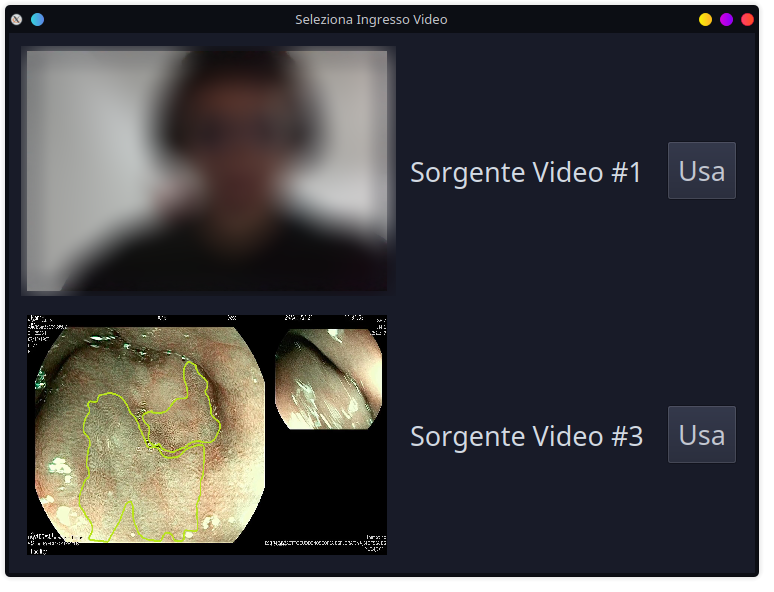
\includegraphics[width=0.9\textwidth]{./assets/app-splashscreen.png}
    \caption{\label{fig:app-splashscreen} Finestra selezione ingresso video}
\end{figure}

Questo passaggio è necessario poiché non è noto a priori
quale sia l'ID dello strumento utilizzato dal personale medico,
che dipende dall'ordine in cui i sistemi operativi assegnano
questo ID all'accensione e al momento in cui il dispositivo
viene collegato al computer.
Per scegliere una sorgente video è sufficiente premere
il bottone {\tt Usa} accanto al suo ID, e per facilitare
tale operazione una piccola anteprima in tempo reale
viene mostrata in corrispondenza di ogni sorgente video
disponibile, come visibile in figura \ref{fig:app-splashscreen}.

Questo step esclude dal processo di selezione le sorgenti video
non valide o non disponibili.
Sempre in figura \ref{fig:app-splashscreen} infatti notiamo come
siano disponibili le sorgenti video 1 e 3, che corrispondono
ai dispositivi video 0 e 2, siano riportati in questa
finestra di selezione, mentre il dispositivo 1 e di conseguenza
la sorgente video 2 non è selezionabile.
Questo accade perché nella postazione di sviluppo dell'interfaccia
il dispositivo 1 è in realtà un'interfaccia virtuale del
dispositivo 0 e come tale non puo' essere impiegata per
l'acquisizione di immagini.

Selezionando una delle opzioni la finestra viene quindi chiusa
e si apre una seconda finestra che mostra il video selezionato
e dà l'accesso alle funzionalità dell'applicativo.
Da questo momento l'applicativo è gia in funzione
e al di sopra dell'uscita video vengono mostrare le predizioni
del modello.
Gli unici ulteriori controlli che l'utente puo' modificare a
suo piacimento sono degli {\it slider} che permettono di
regolare due parametri delle predizioni, che sono
l'opacità e lo spessore della maschera creata.
Questi due parametri sono stati resi modificabili in modo
da poter scegliere una combinazione che risulti
in maschere di predizioni visibili in modo chiaro e allo
stesso tempo che non coprano porzioni troppo elevate di
immagine o siano troppo distraenti.


